\chapter[Virtual Memory]{Virtual Memory \\ \Large \textnormal{Group Milestone}}

\section{Introduction}

The memory allocator handles the management of physical memory. With it we can allocate and free chunks of physical memory. However it is not possible yet to write specific content to them and read from them as they are not mapped in the virtual address space.

\subsection{The virtual address space}

As for most operating systems, each running process in our operating system has its own virtual address space. The virtual address space is defined using a page table which given a virtual address returns a physical address or tells that this virtual address is not mapped to any physical storage.

\medskip

The page table works as follows. There are page tables of multiple hierarchical levels. Each page table can be seen as an array of 512 ($2^9$) page table entries for the first three levels or an array of frames capabilities for the last level. The first level, which is the L0 level, can be seen as a structure that allows to point to up to 512 L1 page tables. This is analogous for the L1 and L2 table entry pages. They keep in memory pointers to respectively L2 and L3 page tables. A L3 page table has frames in memory.
\medskip
When using only 4KB pages, meaning that we only map chunks of 4KB of physical memory at a time, with Aarch64, only 48 bits (out of 64) of the virtual address are used. 
The first 9 bits correspond to the index L0, the 9 following give the address L1, the 9 following the address L2 and the 9 following the address L3. The last 12 bits correspond to the offset in the 4KB physical memory page.

\begin{figure}
    \centering
    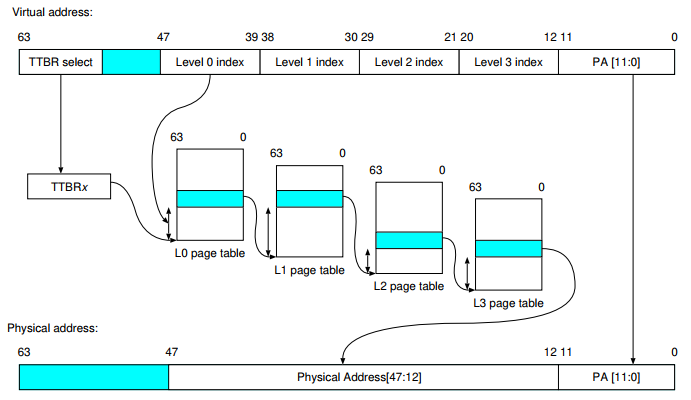
\includegraphics[scale=0.6]{images/memory/page_table.png}
    \caption{ARMv8-A page table with 4KB pages}
\end{figure}

\section{Page fault and lazy paging}

We can remark that storing page tables for all possible entries and levels would require $2^36$ * sizeof(entry) byte which would be way to much. A way to circumvent that is to specify for each level in each valid table if an entry is valid or not. If it is not valid, this means that the whole virtual memory range backed by this entry is not mapped so we do not have to store the underlying higher level page tables and entries.

In the event where we access a virtual memory address which is not backed by physical memory, during the physical address resolution, the index pointing to the next page table level or frame will be invalid. In this cause, an exception called page fault will be triggered. The Barrelfish micro-kernel catches this page fault and allows us to define a page fault handler which will be called in this case. The page fault handler can then be used to map physical memory at the virtual address location which triggered the page fault and then the process can resume as if nothing happened.

This allows us to use the concept of lazy paging: the virtual memory allocator can mark some memory pages as lazily allocated: there is not any physical memory backing it but as soon as we try to read or write from it, the page handler will in a transparent way map memory when necessary.
As such, if we lazily allocate 10GB of memory but only use 16MB of it, only 16MB of physical memory will get allocated and the process won't suffer from insufficient memory.



\section{Mapping Memory}

Apart from using a Red-Black Tree to handle the virtual address space, as explained earlier, it is crucial for us to monitor and consistently update the mappings to the \emph{physical address space}.

In our implementation, we opted to keep track of a process' mappings in a data structure closely resembling a \href{https://en.wikipedia.org/wiki/Shadow_table}{Shadow Page Table}, as shown in Listing \ref{listing:shadow_pt}. As part of our \texttt{paging\_state}, we thus keep track of the \emph{root level} page table.

Whenever we update a process' virtual address translation via the MMU, we update our internal mapping correspondingly. This ensure that the Shadow Page Table is kept up to date throughout any mapping/unmapping performed as part of \texttt{paging.c}.

\begin{lstlisting}[caption={\texttt{page\_table}: Keeping Track of Memory Mappings},label={listing:shadow_pt}]
struct page_table {
   enum objtype type;           ///< type of the page table
   uint16_t index;              ///< index in the parent page table 
   struct capref page_table;    ///< page table capability
   struct capref mapping;       ///< mapping capability

   /// entries within the page table
   union page_table_entry {
       struct page_table *pt;   ///< if type != L3
       struct capref frame_cap; ///< if type == L3 (mapping)
   } entries[VMSAv8_64_PTABLE_NUM_ENTRIES];
   
   /// "bit-array" indicating lazy allocation (if type == L3)
   int32_t lazy[(VMSAv8_64_PTABLE_NUM_ENTRIES + 32 - 1) / 32];
   
   ///counts the number of non-NULL children
   uint16_t num_children;
};
\end{lstlisting}

We chose this particular data structure because it strikes an excellent balance between efficiency and simplicity. Since nearly all upcoming milestones rely on the functionality provided in paging.c, it is imperative that we ensure its efficiency, reliability, and ease of debugging. Looking back, this decision has turned out to be incredibly valuable. During our development process, we encountered intricate bugs within our paging implementation that would have been significantly more challenging to debug if we had chosen a more complex data structure.


\subsection{Mapping a Frame}

We must provide the following functions to map a frame:
\begin{lstlisting}[caption={Mapping a Frame}]
errval_t paging_map_frame_attr_offset(struct paging_state *st, void **buf, size_t bytes, struct capref frame, size_t offset, int flags);

errval_t paging_map_fixed_attr_offset(struct paging_state *st, lvaddr_t vaddr, struct capref frame, size_t bytes, size_t offset, int flags);
\end{lstlisting}

Both functions are conceptually very similar. For \texttt{paging\_map\_frame\_attr\_offset} we may map the frame to any virtual address, where as the caller explicitly provides a desired virtual address as part of \texttt{paging\_map\_fixed\_attr\_offset}.

Our implementation reflects the similarity between the two functions. In both cases, we first perform the corresponding function to allocate the required virtual address space. Subsequently, we traverse our Shadow Page Table, allocating and initializing any child (shadow) page tables, if required.

In cases where mappings extend across multiple pages, we can easily handle them by iterating over the address space and mapping the frame with the appropriate offset. However, if the span of the mapping fits within a single leaf page table, we can avoid repeating the process of traversing the entire recursive mapping. It is worth noting that, in line with our objective of facilitating efficient debugging, we made a deliberate decision not to explicitly handle these specific edge cases, instead we always traverse the entire root to leaf mapping.

For the purpose of lazy allocations, we additionally support:
\begin{lstlisting}[caption={Mapping a Frame (Lazy)}]
    errval_t try_map(struct paging_state *st, lvaddr_t vaddr);
\end{lstlisting}
In particular, \texttt{try\_map} does not map the entire region, instead the mapping is performed lazily in this case. Here, we look up the virtual address allocation containing the provided \texttt{vaddr}, and make sure to map it. Furthermore, we make sure to set the corresponding bit in the \texttt{lazy} bit-array, as captured in Listing \ref{listing:shadow_pt}. This ensures that we can perform the necessary steps for lazily allocated regions during unmapping. 

\subsection{Unmapping a Frame}

\texttt{paging\_unmap} is used to unmap a previously mapped frame:
\begin{lstlisting}[caption={Unmapping a Frame}]
    errval_t paging_unmap(struct paging_state *st, 
                          const void *region);
\end{lstlisting}

Unmapping frames is conceptually very similar to mapping them. We find the virtual address region belonging to the provided \texttt{region} pointer, and then traverse our Shadow Page Table undoing any previously performed mappings. At the leaf level, we make use of the previously introduced \texttt{lazy} bitset. If the corresponding frame was allocated lazily, we make sure to also \texttt{cap\_destory} the corresponding frame. Finally, we free the corresponding allocation in the virtual address space. Once again the unmapping of regions spanning multiple pages is done by iterating over every contained page.

We additionally provide
\begin{lstlisting}[caption={Mapping a Frame}]
errval_t paging_decommit(struct paging_state *st, lvaddr_t vaddr, size_t bytes);
\end{lstlisting}
for the purpose of unmapping the corresponding region, while preserving the allocation in the virtual address space.

\subsection{Handling a Page Fault}

There are two main components that can be adjusted to decide how a page fault will be handled.

The first of these is the exception handler stack. While it may seem that the simplest solution would be to simply continue using the same stack when an exception occurs, this solution has a significant fault: Each thread's stack is also dynamically allocated, and not fully backed by memory. This means that, if the exception handler used the same stack as the rest of the program, it might run into a page fault while handling a page fault (which would terminate the execution of the program). Instead, we maintain a slab allocator which manages smaller, but fully mapped, slabs of memory to use as exception handler stacks. When a thread is created, its exception handler stack is allocated from this pool. This guarantees that no exceptions occur while handling an exception.

The second is the actual page fault handler function, which is called \texttt{\_paging\_handle\_exception} in our implementation. The function is conceptually very simple:
When a page fault occurs, we identify the associated virtual address space allocation and proceed to map it using the \texttt{try\_map} function, ensuring there is adequate space available in the slab allocator.

To facilitate more precise debugging, we deliberately trigger a panic if we encounter any address resolution within the first \texttt{BASE\_PAGE\_SIZE} bytes, as this usually implies a \texttt{NULL} pointer dereference.

Both the handler function and the exception handler stack are set up before a thread begins executing its target function.

\begin{comment}
We talked only about using 4KB pages. However, there are different page sizes available. For example, we could store directly a frame in a L2 page table entry. The frame will then be a 2MB page. We did not implement huge pages in our OS.
\end{comment}

\begin{comment}


Virtual memory manager

Allocating virtual memory

Different class of allocators

Red black trees

Paging

Why paging
Currently we have two memory managers. The first one is responsible for distributing physical memory (ram capabilities) to each process according to its needs. Once a process no longer needs memory, it can give it back and be used by another process. As far as virtual addressing is concerned, i.e. the address that the process sees, we have an ad-hoc memory allocator. However, there is still an open question. How to connect the virtual addresses to the physical addresses that represent the addresses in the ram. In order to solve this problem, we need a mechanism to translate in some way a virtual address into a physical adress. There is a technique to solve this problem. This technique is named paging.

What is paging exactly ?
Paging is a technique to translate a virtual address into a physical address. The processor maintains a data structure called a page table which will allow him to translate each virtual address into a physical one. When the processor reads a virtual address, it translates it and then reads the contents in memory of the translated physical address.

How does it work.

TODO : Add figure here

How did we implement it

How to implement it in practice

Memory request for a process:
When a processor needs memory, the operating system will request the virtual address. Our operating system will then request a physical address segment in the background and modify the page table data structure to translate the virtual addresses returned to the physical addresses returned by the allocator. To do this, we have two mechanisms to do it. The first is called eager allocation and the second is called lazy allocation.
The eager allocation works as follows. The operating system requests physical memory. It then requests virtual memory and directly builds the corresponding entries in the table entry page. This is the method used in our page_attr_offset function (todo: give good function name). If we assume that the page table will never be modified, we have by definition no page fault in the system. All the overhead of the installation is done at memory allocation time.
// TODO MAKE A SMALL SCHEME eager mapping
Lazy allocation works differently. When the process requests memory, the operating systems will ask the physical memory manager for a frame of the corresponding size and a segment in the virtual address. The operating systems does nothing else for the moment. Each time the program tries to translate and the page is not present, it will trigger an interrupt that corresponds to the page fault. At this point, the operating will perform the mapping "on the fly".

\end{comment}


\section{Virtual memory allocator}

\subsection{Role of the virtual memory allocator}

At this moment, we have the infrastructure to map and unmap pages, which allows us to bind the virtual address space to the physical addresses provided by our system and the capabilities. This is an essential step in the overall process, but it is only half of the work done.

Let's imagine we have the code that starts, stops, ends, and resumes a process. However, there is still an important question to answer: when should each process be allowed to run and for how long? This is known as a scheduling problem. In simpler terms, even though we know how to perform the mapping process, we haven't decided which specific mappings should happen. The only difference is that, instead of dividing computing power, we need to divide memory resources.

To grasp the concept better, let's consider a scenario where we have a group of tasks waiting to be executed. Each task requires a certain amount of resources, and we have a limited supply of these resources. It becomes essential to \texttt{prioritize} and \texttt{schedule} the tasks effectively to ensure \texttt{optimal resource utilization}.

In a similar manner, when dealing with mapping and unmapping pages in virtual memory, we encounter a similar challenge. We have a pool of virtual addresses and a finite set of physical addresses available for mapping. Our goal is to \texttt{efficiently allocate} these physical addresses to the virtual addresses in a way that maximizes the overall performance and resource utilization of our system.

To accomplish this, we need to develop a strategy or algorithm that determines the most effective mapping sequence. This algorithm would consider various factors, such as the size of the virtual address space, the available physical memory, the priority of the tasks, and any constraints or requirements imposed by the system.

Therefore, while we have the technical capability to perform the mapping and unmapping of pages, the larger task at hand is to devise an intelligent and efficient approach for deciding which specific mappings should be executed in what order. This ensures that the virtual address space is effectively connected to the physical addresses, optimizing the performance and resource management of the system as a whole.

\subsubsection{The choice of the memory allocator}

The task of managing virtual memory allocation is quite similar to managing physical memory allocation. In both cases, we have a set of addresses that we need to assign and release when they are no longer needed. There are various methods to implement a memory allocator, each using different algorithms. However, to simplify the process, we have two choices to consider.

One option is to start by implementing a simple allocator using a \texttt{linked list}. This approach would be easier to implement compared to more complex algorithms. With this allocator, inserting and freeing memory can be straightforward in the best-case scenario. However, as the number of allocated nodes increases, the operations become linear in nature. In other words, the performance of the system gradually decreases with multiple allocations, which is not an optimal outcome.

While the \texttt{linked list allocator} may be easy to implement initially, its performance shortcomings make it less ideal in the long run. It becomes apparent that a different approach is needed to achieve optimal memory allocation.

To address this limitation, we can explore other advanced algorithms such as \href{https://en.wikipedia.org/wiki/Binary_tree}{\texttt{binary trees}}, \href{https://www.cs.auckland.ac.nz/software/AlgAnim/red_black.html}{\texttt{red-black trees}}, or \href{https://en.wikipedia.org/wiki/Hash_table}{\texttt{hash tables}}. These data structures offer more efficient ways of managing memory allocation. For instance, binary trees enable faster search operations, while \texttt{red-black trees} provide a \texttt{balanced structure} that ensures efficient insertion and deletion operations. Hash tables, on the other hand, offer constant-time access to memory blocks, making them highly efficient.

By implementing one of these more advanced memory allocators, we can overcome the limitations of a simple linked list approach. These algorithms allow for improved performance even with multiple allocations, ensuring that the system operates at an optimal speed and efficiency.

After considering various options, we have chosen to implement a \texttt{red-black tree} for our memory allocator. This algorithm is more complicated to write and has a higher risk of bugs compared to a simple linked list. However, when it comes to performance, the \texttt{red-black tree} outshines the \texttt{linked list allocator}.

The key advantage of using a \texttt{red-black tree} is that its running time is \texttt{logarithmic}. This means that as the number of allocated nodes increases, the time it takes to perform operations like insertion and deletion grows much slower compared to a linearly increasing time in a \texttt{linked list}. In simpler terms, the \texttt{red-black tree} allows us to allocate and free memory blocks efficiently, resulting in faster processing overall.

In practical terms, implementing the \texttt{red-black tree} allocator means that our system will experience less overhead in memory allocation over time. This is because the performance of the \texttt{red-black tree} remains stable even as the number of allocated nodes grows. As a result, processes relying on memory allocation will suffer less from the associated delays and inefficiencies, leading to smoother and faster execution.

Although the \texttt{red-black tree allocator} requires more effort to implement and carries a higher risk of bugs, the long-term benefits in terms of performance make it a worthwhile choice. The trade-off between complexity and efficiency is justified by the significant improvement in running time and reduced overhead experienced by the system as a whole.

\subsubsection{The implementation of the red-black tree}

Each node in the tree represents a virtual memory range which can be used or free and they are ordered using their virtual memory range, as they don't overlap. Using a balanced binary tree allows us to do the following operations in \texttt{worst-case logarithmic time}:

\begin{itemize}
    \item \verb|Insert|(T, u): Insert node u in the tree T, effectively adding a new memory range to the tree
    \item \verb|Remove|(T,u): Remove node u from tree T, removing a managed range from the tree
    \item \verb|Pred|(T,u): Find the memory range before the one managed by u
    \item \verb|Succ|(T,u): Find the memory range after the one managed by u
    \item \verb|Find|(T, r): Find the memory range containing the virtual address r
\end{itemize}


\begin{lstlisting}[caption={The red-black tree node},label={listing:shadow_pt}]
/// @brief A node in the red-black tree, if in the tree, its fields should only be read
/// The field start can be modified given that it does not modify the node position relative
/// to the other nodes. The field size should only be modified using the rb_tree_update_size method
/// The max_size field is automatically maintained
struct rb_node {
    struct rb_node *parent;
    struct rb_node *left;
    struct rb_node *right;

    lvaddr_t start;
    size_t   size;

    size_t max_size;
    bool   is_red;
};

/// @brief An augmented red-back tree
struct rb_tree {
    struct rb_node *root;
};
\end{lstlisting}


\begin{lstlisting}[caption={Functions availables in the red-black tree},label={listing:shadow_pt}]
// Initialize the red-black tree, call before using the tree for the first time
void rb_tree_init(struct rb_tree *tree);

// Insert a node in the tree
// z should have been externally allocated and have its start and size fields already set
void rb_tree_insert(struct rb_tree *tree, struct rb_node *z);

// Remove a node from the tree
// z should point to a node already in the tree
void rb_tree_delete(struct rb_tree *tree, struct rb_node *z);

// Return the node containing the given address or NULL if none was found
struct rb_node *rb_tree_find(struct rb_tree *tree, lvaddr_t addr);

// Return a node of size at least size or NULL if none exists
// A worst-fit strategy is used
struct rb_node *rb_tree_find_minsize(struct rb_tree *tree, size_t size);

// return the first node wich starts at an addres greater or equal to addr
// or NULL if no such node exists
struct rb_node *rb_tree_find_greater(struct rb_tree *tree, lvaddr_t addr);

// return the first node wich starts at an addres lower or equal to addr
// or NULL if no such node exists
struct rb_node *rb_tree_find_lower(struct rb_tree *tree, lvaddr_t addr);

struct rb_node *rb_tree_successor(struct rb_node *node);

struct rb_node *rb_tree_predecessor(struct rb_node *node);

// Update the size of a node, without having to remove and re-insert it
void rb_tree_update_size(struct rb_node *node, size_t size);

// Helper function to check if a tree was corrupted
// Return true if the tree is fine
bool rb_tree_check(struct rb_tree *tree);

// Print the content of the tree using debug_printf
// The nodes are printed using an inorder walk
void rb_tree_print(struct rb_tree *tree);

\end{lstlisting}

Moreover, the tree is augmented with a \verb|size| attribute. This field gives for each node the size of the largest contiguous free virtual range in the subtree rooted at this node. Using this, we can immediately know for a given size if there is enough contiguous space to map it and makes implementing a worst-fit strategy for the memory allocation really easy. This data structure can also be used to allocate at a fixed location or tell that it is not possible.

\section{Morecore implementation}

The \texttt{malloc} function used to dynamically allocate memory internally calls a \verb|morecore| function when it requires more memory. We want the memory returned by multiple calls to morecore to be as often as possible contiguous to decrease fragmentation when alternating between malloc and free. This is a perfect use case for the lazy paging approach.

When morecore gets called, a 256GB contiguous memory range gets reserved, then we use a linear allocator in it to return memory. Thanks to lazy paging, only the range that gets used will actually be physically backed by memory and doing so, we reduce fragmentation. There are of course special cases if we malloc more than 256GB of memory at once (just reserve a memory range that is big enough) or overall more than 256GB (reserve a new 256GB memory range and switch to it).

\section{Retrospective}

When we look at how important the virtual memory allocator is in Barrelfish, just like its physical memory allocator counterpart, the most important thing is that it works reliably. Any mistake can (and did) lead to hard-to-debug issues later. 

In terms performance, our virtual memory allocator has shown less problems over time compared to the physical memory allocator. This is expected, as it uses a data structure with logarithmic time complexity, while the physical memory allocator has linear complexity in the worst case.
